

%%%%%%%%%%%%%%%%%%% Section 8 %%%%%%%%%%%%%%%%%%%%%%%
\IEEEraisesectionheading{\section{Introduction}
\label{sec:introduction}}

\IEEEPARstart{B}{ackbone} structures \cite{cheng1998development,nick2013simmelian} are well established
to understand the connectivity and relationships among critical entities in networks.
Consider a network $G$ and a set $V_I$ of
nodes of interests designated by
users. One often wants to understand the relationships among
$V_I$ by finding a {\em backbone} $T$, \ie a subtree of $G$ that spans
over $V_I$ 
with a minimized connection cost.
Backbone detection has been applied for Pathway identification in biology study \cite{bailly2011finding}, information propagation \cite{kumar2017information}, and
network flow optimization\cite{kumar2012optimization}.

\vspace{.5ex}
Emerging needs in understanding
richly attributed networks require the
detection of new type of backbones. In 
these backbones, 
each edge and its semantic is dynamically
characterized 
by {\em specific attributes and
values} of its end nodes. Moreover, these 
attributes and their values also provide intuitive interpretation
for the backbone structures.
 %%%%%%%%%%%%%%%%%%%%%%%
Consider the following example.

\begin{example}
\label{exa-motivate}
Fig.~\ref{fig:backboneex} illustrates a fraction of an attributed geo-social network $G$. Each node $v$ in $G$
is a landmark with properties such as \texttt{type} 
or \texttt{location},
as well as attributes from statistics of
its past visitors, such as major \texttt{gender} (\eg `female'), \texttt{tour\_type} (\eg `family'), or
type of favored attractions
\texttt{attr\_type} (\eg `museum')
when stayed at $v$. Such information
can be extracted from 
photos, check-in or review data~\cite{cheng2011personalized}.
The edges denote routes among
the landmarks. % in $G$. 

\eat{
\reviseS{In the traditional personalized trip recommendation work~\cite{lim2015personalized}, the user needs to specify her destination Point of Interest (\poi) in order to return a personalized path. However, it is difficult for a user to narrow down to a potential set of \poi{s} and to specify a destination. In this case, a tree structure is helpful to give the user a recommendation backbone that helps her further locate the starting \poi and the destination \poi and extract a path from this backbone.}
}

To identify potential tours in $G$ from scratch without 
knowing specific destination, a 
user may want to start with a ``backbone'' (a tree)
with a root (\eg $v_1$ (hotel)) that 
spans a set of point of interests (\pois) 
to further inspect specific trips. 
Moreover, she may want to pose specific constraints 
as``\texttt{tour\_type}'' or ``\texttt{attr\_type}'' 
to enforce that each route connects landmarks 
favored by similar type of tours (\eg 'family') or have similar type (\eg 'museum'), 
respectively. 
As such, 
the significance of each route in a tour %$T$ 
varies due to different focus of preference
reflected by specific
attributes and their values. 
%Consider the following two cases. 

%Personalized trip recommendation aims to
%compute backbones $T$ that span a set of
%attractions (marked by red nodes)
%with a root $v_1$ (hotel). 

%\reviseS{A user can identify a set of attributes that attracts her first, such as tour type \texttt{tour\_type} (\eg `family') or type of favored attractions \texttt{attr\_type} (\eg `museum').}
%The significance of a route in $T$
%may vary due to different focus of preference
%reflected by specific
%attributes and their values.
\sstab
(1) When a user
specifies attribute ``\texttt{location}'', 
the connection cost of
routes between two landmarks should be measured by 
geographical distance. For example, 
a route from restaurant $v_4$ to attraction $v_5$
(from coordinates $(150,200)$ to $(150,175)$) 
has smaller cost under ``\texttt{location}''. 
The route $(v_5, v_{12})$ is relatively less favorable
due to longer distance ($(150,175)$ to $(180,70)$). 

\sstab
(2) Another user may prefer tours that
connect attractions
featuring similar ``family tours'' (\texttt{tour\_type}).
The same route $(v_4, v_5)$
under this specification % of tour type
becomes less desirable compared with
route $(v_5, v_{12})$ that connects two
attractions both featuring family tours.
Indeed, $v_4$ and $v_5$ are not
``close'' as $v_4$ is
more favored by ``couple''.

\vspace{.5ex}
A recommended tour that carries
attributes on its routes 
indicate the rationale of the
recommendation. For the first user,
a trip plan (colored in blue)
suggests that ``{\em Park $v_2$, Museum $v_3$ and
restaurant $v_4$ are closer as
they are favored by the same gender group
``female'', while the rest suggest
closer trips}. The second plan (colored in orange)
are more favorable to family tours.
Moreover, it is desirable to suggest trips along with the geo-social attributes
that determine their cost,
when users are not familiar with
underlying data.
\end{example}

\begin{figure}[tb!]
\centering
\centerline{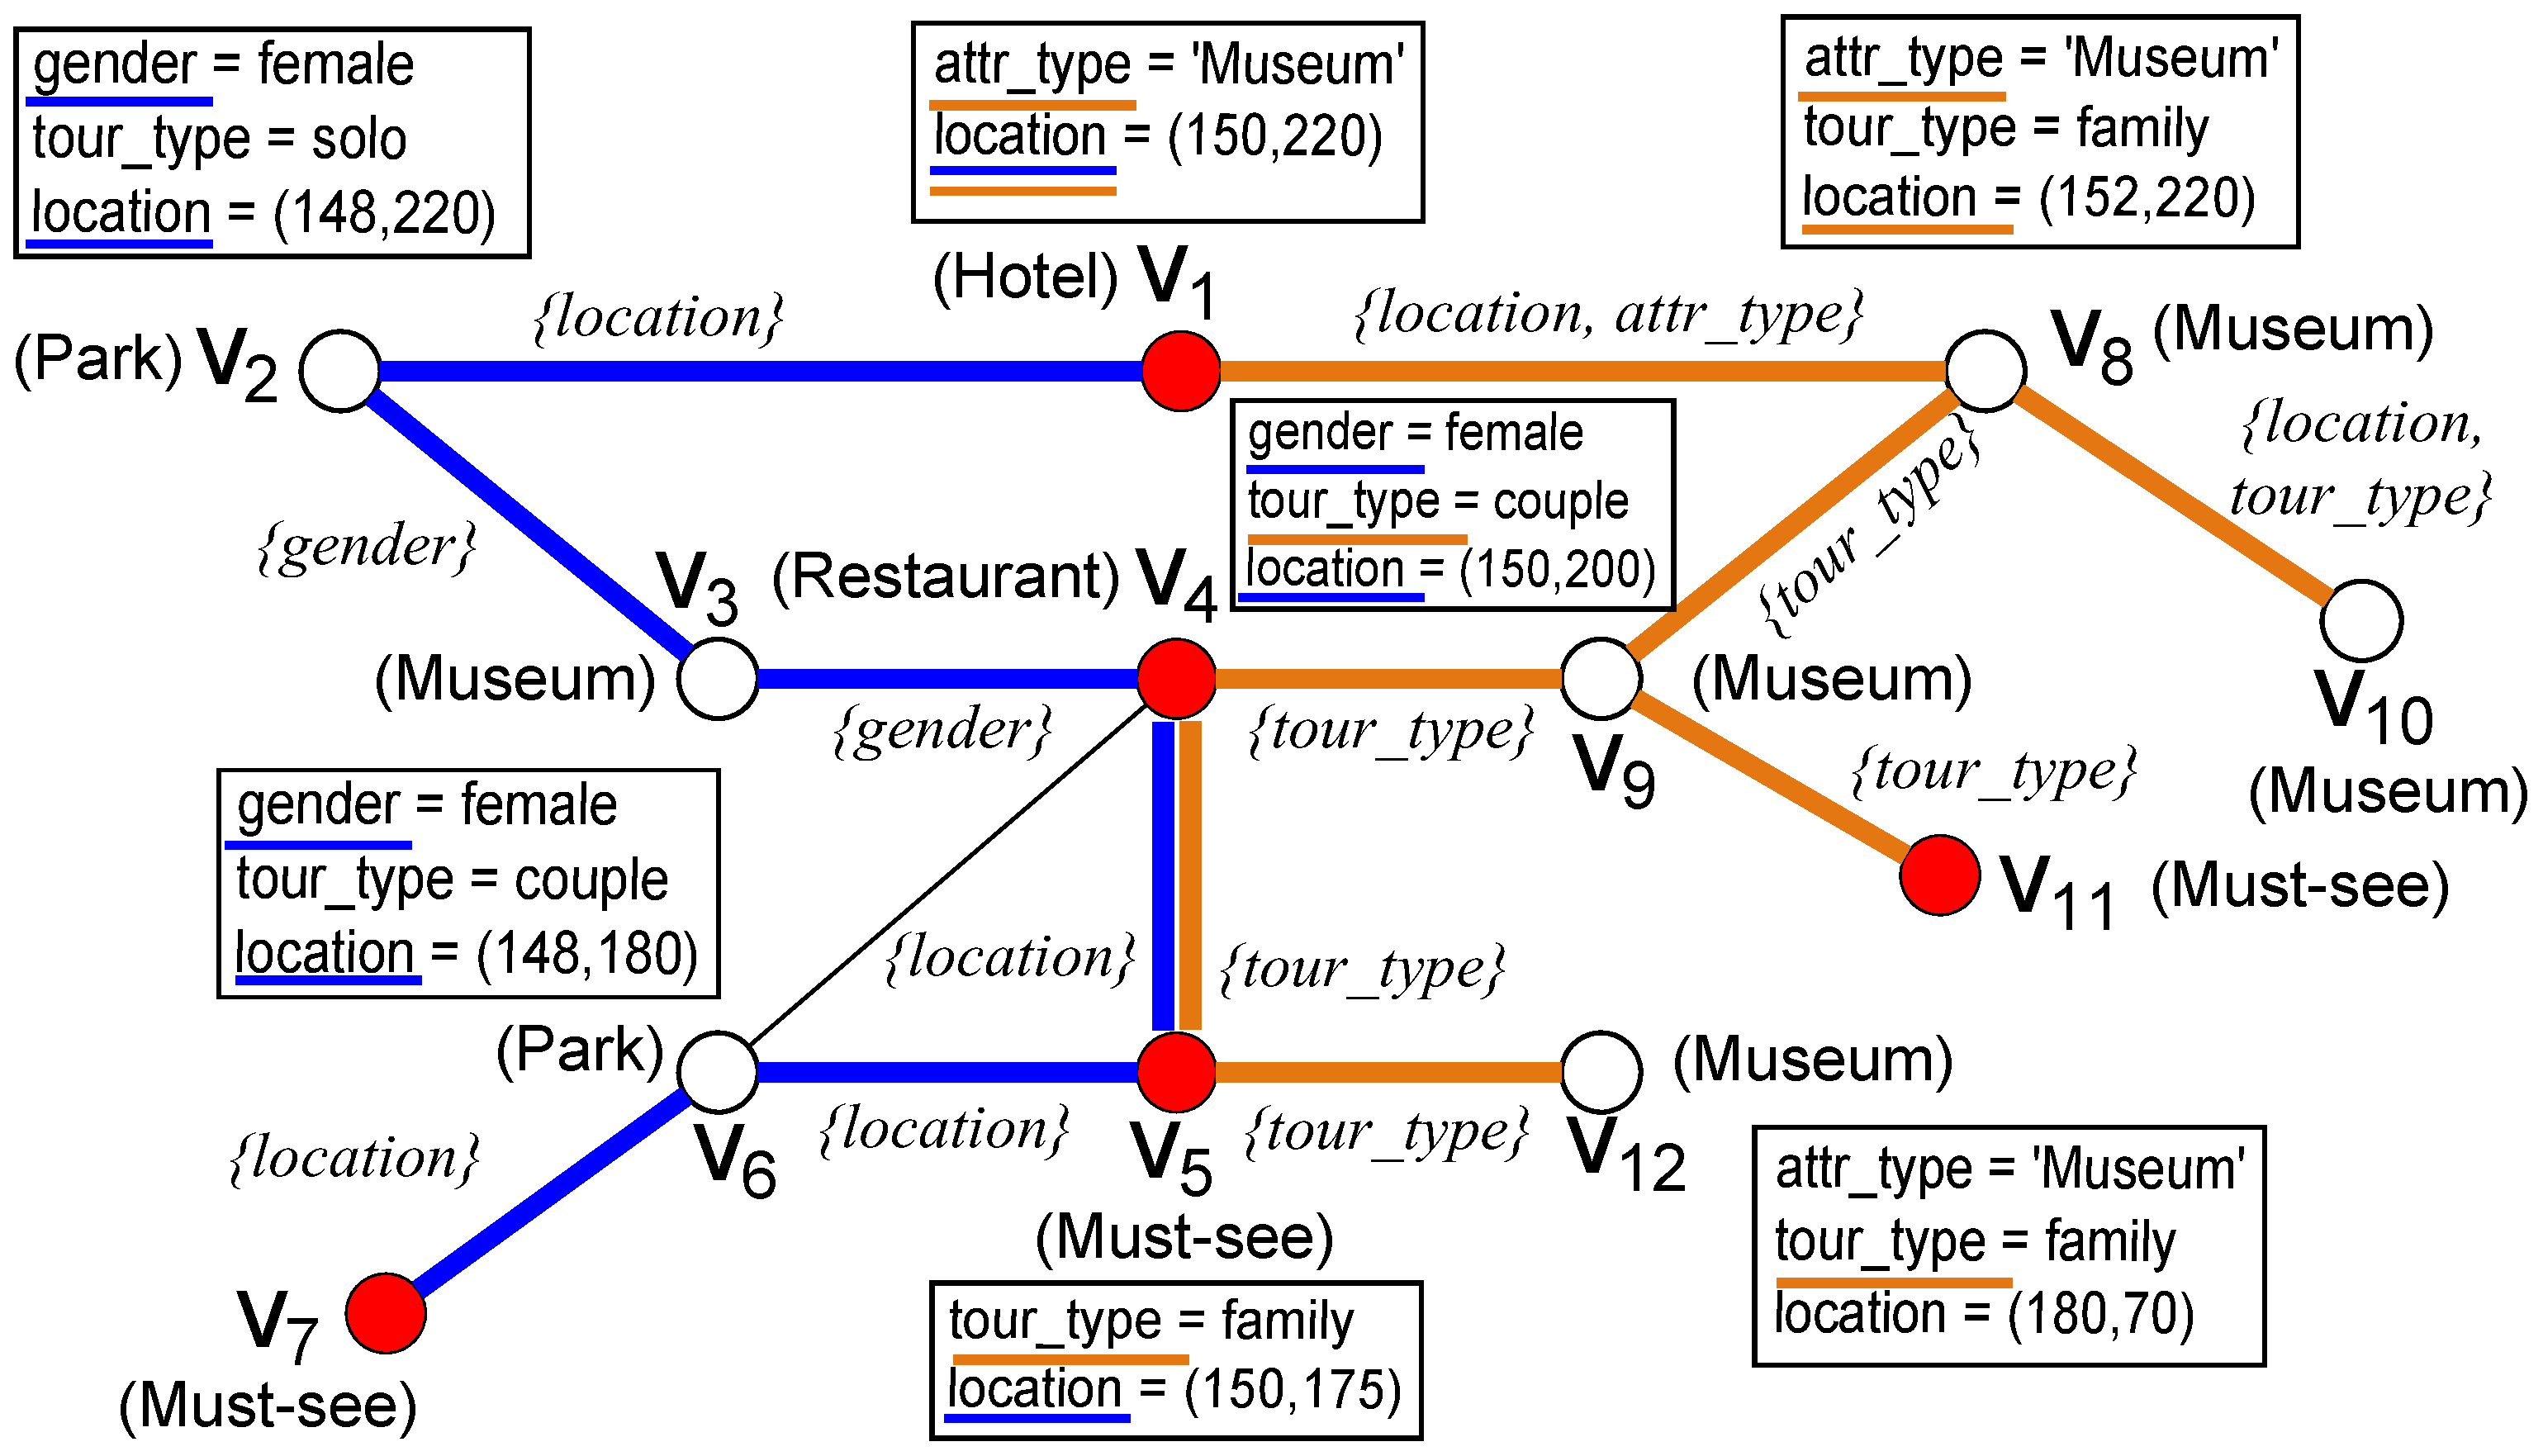
\includegraphics[width=0.5\textwidth]{./fig/Fig1-backbone-example.eps}}
\caption{Suggesting tours %as backbones
 with geo-social attributes.
}
\label{fig:backboneex}
\vspace{-2ex}
\end{figure}


The above scenario is a departure from conventional 
trip recommendation that assumes 
a fixed cost model and known destinations. 
The backbone structures in the example, although
desirable, cannot be characterized by 
conventional characterization such as
Steiner trees~\cite{chiang2013steiner}. 
Indeed, these backbones are
{\em jointly characterized} by
interesting nodes and
their relationships as well as
the connectivity cost determined by
specific node attributes of interests. 
%\reviseS{Attributes associated on each edge are affinitive attributes.}

\vspace{.5ex}
We call such backbone structures
{\em attribute-driven backbones}.
Attribute-driven backbones 
can be characterized by
a weighted tree $T$ = $(V_T, E_T)$ that connects a set of attributed nodes $V_T$,
where
each edge $e$=$(v, v')$ in $T$
is associated with a set of {\em affinitive attributes} $A$, such that both $v$ and $v'$ 
carry non-empty values
for each attribute in $A$.
\eat{It intuitively states that
the significance of edge $e$ (\eg \blue{the edge weight between two Weibo tweets} )
is determined by relevant attributes
$A$ (\eg \blue{publishing time, the number of retweets, hash tag keywords, description, etc.}), and quantified by its values
from both $v$ and $v'$ (\eg \blue{the publishing time of these two tweets, keywords in hashtag of these two tweets, etc.}).
}
%The intuition is that
The cost of an edge
$e$ in $E_T$ should be dynamically determined by
the selection of its affinitive attributes
and their values. 

\stitle{\warn{A new motivation for the online attribute driven backbone needs to be put here}}

%\reviseS{After a backbone $T$ is obtained, the user can choose two nodes as starting and destination \poi and apply pathfinding algorithms, such as Dijkstra's algorithm in this backbone $T$ to find a path.}

\vspace{.5ex}
We study a new problem called
{\em attribute\eat{d}-driven backbone discovery} (\abd),
characterized as follows.
\tbi
\item \textbf{Input}: Attributed graph $G$, a set of interested nodes $V_I$ in $G$,
an interestingness function $I$, and an edge cost model $C$ that assigns a weight
to an edge given its affinitive attributes;
\item \textbf{Output}: an attributed backbone $T$ that connects
the nodes in $V_I$ with maximized interestingness in terms of $I$, and
minimized edge cost in terms of $C$.
\ei

\stitle{Applications}. 
Attribute-driven backbones readily provide enriched models 
for cascade structures enhanced by affinity attributes 
that may ``explain'' the connectivity between 
entities. 
(1) Attribute-driven backbones in geo-social networks 
can be used to further suggest personalized trips 
(paths) in trip recommendations~\cite{cheng2011personalized}. (2)
  %with applications in 
Signaling cascades such as 
pathways among proteins~\cite{bailly2011finding} 
can be modeled as attribute-driven backbones 
starting at receptor proteins and transmitted through protein interactions to effector proteins. 
The affinity attributes indicate interaction 
patterns between proteins with high confidence. 
(3) Adding affinity attributes to backbones in 
academic networks provide more expressive 
and interpretable collaboration patterns~\cite{newman2004coauthorship} among scholars, where affinity attributes 
such as ``topics'' or ``affiliation'' 
indicate potential collaboration that benefits 
from similar research areas or institutes. 
Attribute-driven backbones also suggest potential community in sparse networks, where density-based
detection may
become overkill~\cite{chiang2013steiner}, 
as verified by our experimental 
study (Section~\ref{sec-exp}).
%the affinity attribute in  can indicate the degree of acquaintance between two scholars, (\eg `co-authorship is stronger than publishing two different papers on the same venue'). The academic backbone suggests potential collaboration in the future.



% collaborative pattern recommendation~\cite{newman2004coauthorship},
%and network optimization~\cite{kumar2012optimization}.
\eat{
\reviseS{In the signaling cascade, an example can be the phosphorylation MAPK kinase pathways that consists a sequential reactions starting at receptor proteins and transmitted through protein interactions to effector proteins. The attributes carried on edges indicate certain interactions between proteins with higher confidence (protein interactions verified in small-scale
experiments or found in many large-scale datasets). In the academic collaboration pattern recommendation, the attribute carried on the edge indicates the degree of acquaintance between two scholars, (\eg `co-authorship is stronger than publishing two different papers on the same venue'). The academic backbone suggests potential collaboration in the future. }
}


\vspace{.5ex}
Although desirable, computing \abd is nontrivial.
Instead of using predefined
functions, the edge cost $C$ in \abd
(thus the quality of backbones) is dynamically determined
by the selection of affinity attributes.
Conventional community detection 
or Steiner-tree based algorithms \cite{chiang2013steiner}
that rely on static cost model
and labeled graphs can not be directly
applied.

\stitle{Contributions}. We study feasible models and algorithms
to compute {\em attribute-driven backbones} in large attributed networks.

\stab
(1) We formulate attribute-driven backbones to enrich 
the connectivity model among the nodes of interests (Section~\ref{sec-pre}).
We develop a bi-criteria cost model to characterize
good backbones. Unlike conventional models, 
the cost model incorporates both
node interestingness and edge cost, and 
is dynamically determined by the specification of 
affinity attributes and the 
topology of the backbone.

\stab
(2) Based on the cost model, we
formulate the problem of
{\em attributed backbone discovery} problem (\abd) (Section~\ref{sec-problem}).
This problem is
\NP-complete, and is also hard to approximate (\APX-hard).
This result is robust for
polynomial-time computable
cost models.

\stab
(3) Despite the hardness, we show that
\abd is within reach by feasible approximation algorithms.
We show that \abd is {\em fixed-parameter approximable},
under a practical case that the number of node attributes is small.
We develop a {\em Lagrangian preserving $2$-approximation}.
This algorithm specializes a general Goemans-Williamson optimization scheme of
cut problems for \abd. To reduce the cost, we devise a dynamically
maintain {\em frontier} structure that prioritizes and
explores promising edges in the neighbors of
interested nodes in a bi-directional manner (Section~\ref{sec-approx}).

\stab
(4) When the attribute number is large,
we develop a faster heuristic to compute
backbones and relevant attributes. The algorithm
performs a {\em once-for-all} Expectation Maximization (\EM)-based
learning process to identify
a generative model for given attributes, and
grows backbones by iteratively
selecting attributes that can minimize an expected
edge cost for the backbone, for any
given interested nodes (Section~\ref{sec-em}).

\stab
(5) Using real-world graphs, we experimentally verify
the efficiency and effectiveness of our approximation and
heuristic algorithms. We show that our algorithms
can efficiently identify meaningful structures along with relevant attributes that cannot be expressed by
existing backbone models. They also benefit the discovery of potential community structures
in sparse and richly attributed networks
(Section~\ref{sec-exp}).

\stitle{Related Work}. We categorize the related work as follows.

\etitle{Attributed community search}.
Clustering-based community detection has been studied for attributed networks~\cite{bothorel2015clustering,falih2018community}.
I-Louvain method \cite{combe2015louvain}
exploits (categorical and numerical) attributes and topological information
simultaneously.
Index structures are developed~\cite{huang2017attribute}
to further reduce detection cost. ACQ with input $k$~ \cite{fang2016effective} is a subgraph that satisfies both structure cohesiveness ($k$ core) and keyword cohesiveness.
CESNA~\cite{yang2013community} models the dependence and interaction between the network topology and the node attributes and identify
overlapping communities in networks.
While prior work identifies communities (node sets) such that all the nodes in a community share same
set of attributes, we compute backbones
that allow each edge to have its own affinitive attributes. We consider backbones with cost that are dynamically determined by specific selection of affinitive attributes. Prior work typically assumes predefined quality measures that are independent with attributes. We provide approximation algorithms with provable guarantees on the attribute-driven backbones.
On the other hand, the backbones
either reports critical structures in sparse networks
where dense counterparts may not exist, or
benefit the detection of
dense communities~\cite{huang2017attribute}.

\etitle{Connection subgraph detection}.
Connection subgraph detection~\cite{faloutsos2004fast} aims to compute connected (dense) subgraphs that cover source query nodes and incurs a cost under a budget. For example,
\cite{faloutsos2004fast} computes
a subgraph that connects two input
terminal nodes $s$ and $t$ with at most
$b$ nodes, which maximizes the total
network flow from $s$ to $t$. Center-piece
subgraph discovery~\cite{tong2006center}
extends the problem to computing
subgraphs that cover a set of nodes. Detecting dense subgraphs in dual networks \cite{wu2015finding} aims to find a subset of nodes $S$, where two graphs $G_a$ (unweighted) and $G_b$ (weighted) represent physical and conceptual world separately but with complementary information, such that the induced subgraph ${G_a[S]}$ is connected and the density of ${G_b[S]}$ is maximized.  $(k,r)$-core in \cite{zhang2017engagement} represents a cohesive subgraph on social network considering both user engagement and similarity perspectives simultaneously, which contains a $k$-core and an induced clique based on similarity measurement.
These work do not consider node attributes
and assumes predefined edge weights. In contrast, 
the attribute-driven backbones explicitly carry affinitive attributes that suggests the possible ``reason'' of the connection between 
network entities. Moreover, it does not require user to provide 
rigid parameters for topological constraints such as $(k,r)$-core. Posing such constraints can be a daunting task for users and an overkill for detecting community in a sparse network. 
In addition, we develop approximation 
algorithms to discover backbone structures
characterized by attributes.

\etitle{Keyword search in graphs}.
Keyword search over a graph finds a substructure of the graph containing the nodes carrying some or all input keywords
(see~\cite{wang2010survey} for a survey).
Common models include Steiner trees~\cite{kargar2011keyword}
or r-cliques with bounded diameter~\cite{ding2007finding}.
These methods typically
compute a minimum weighted Steiner tree, which is
a special case of \abd with single label, unit node weight and predefined edge weight.
We provide approximation algorithms
to compute more general \abds,
by generalizing Goemans-Williamson scheme~\cite{goemans1995general}
that computes prize collecting Steiner trees
in weighted graphs to attributed networks.

\etitle{\warn{Online backbone-style literature review}}.